\begin{figure}[p]
    \centering
    \begin{subfigure}[b]{0.65\textwidth}
        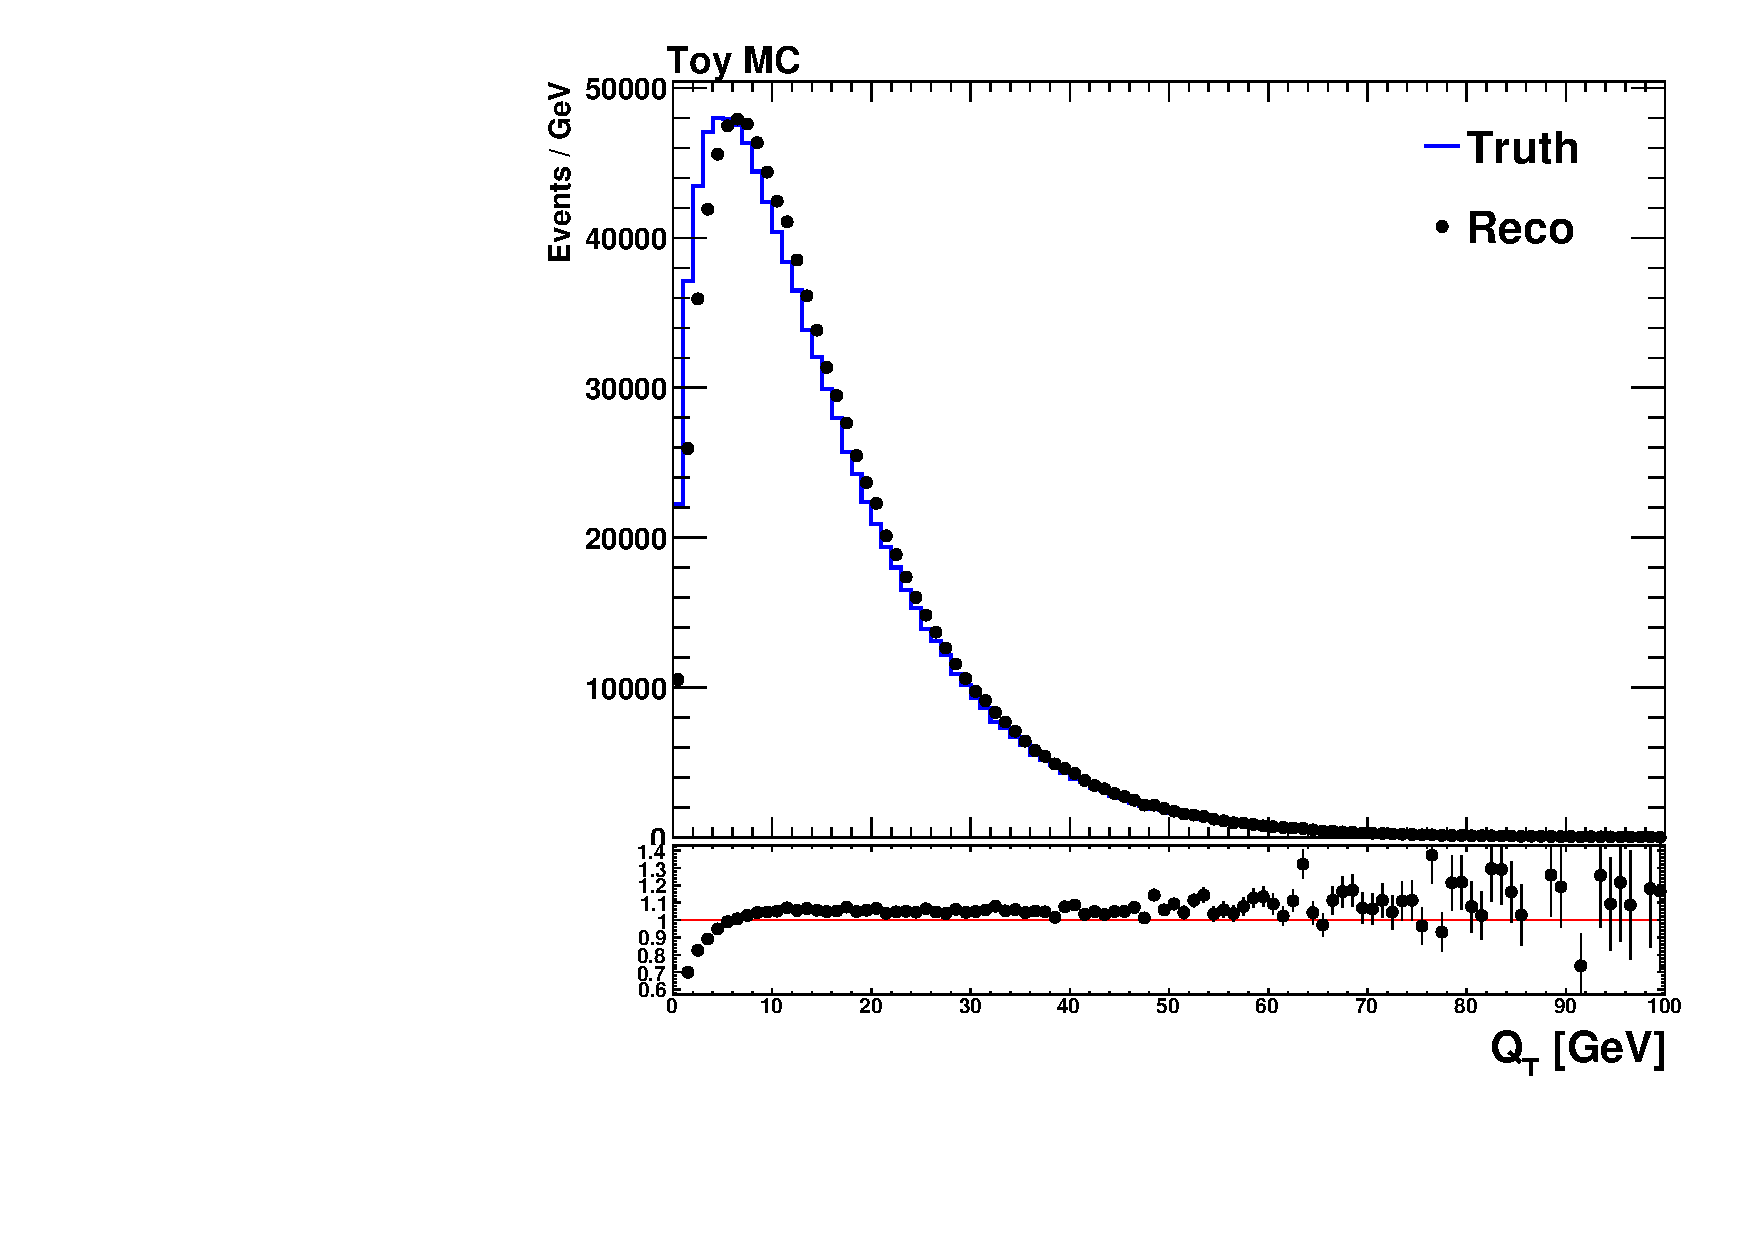
\includegraphics[width=\textwidth]{figures/toy_pt.pdf}
    \end{subfigure}
    \begin{subfigure}[b]{0.65\textwidth}
        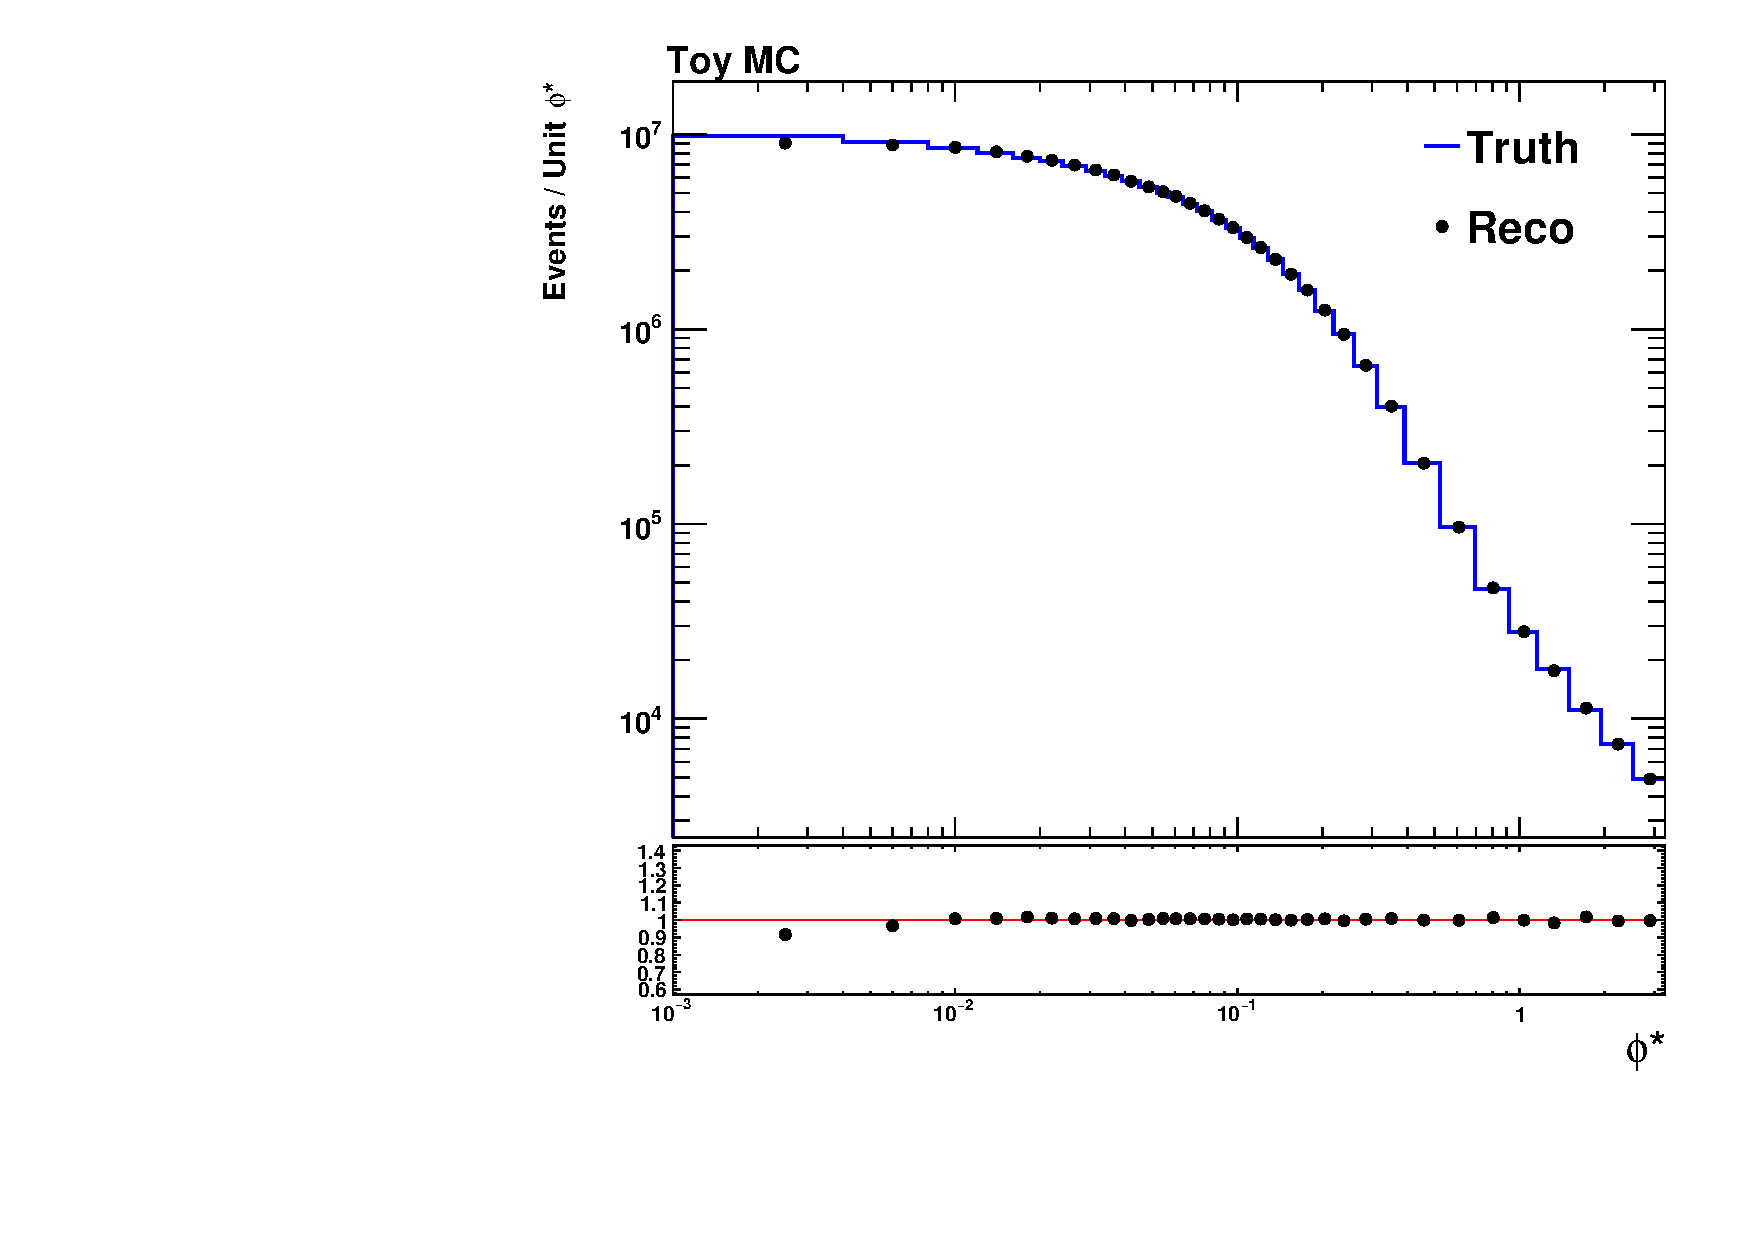
\includegraphics[width=\textwidth]{figures/toy_phistar.pdf}
    \end{subfigure}
    \caption[
        Comparison of \bosonpt and \phistar after smearing.
    ]{
        The top figure shows the \bosonpt distributions as input into a
        simulation (histogram) and as recovered after smearing of lepton's \pt
        (points). The bottom figure shows the \phistar distributions as input
        (histogram) and as recovered after smearing (points).
    }
    \label{fig:toy_phistar}
\end{figure}
